\documentclass[12pt]{article}

\usepackage{scicite,times,graphicx,float,hyperref}
\usepackage[skip=0pt]{caption}

\topmargin -1.0cm
\oddsidemargin 0.0cm
\textwidth 16cm 
\textheight 23cm
\footskip 1.0cm

\newenvironment{sciabstract}{%
\begin{quote} \bf}
{\end{quote}}

\newcounter{lastnote}
\newenvironment{scilastnote}{%
  \setcounter{lastnote}{\value{enumiv}}%
  \addtocounter{lastnote}{+1}%
  \begin{list}%
  {\arabic{lastnote}.}
  {\setlength{\leftmargin}{.22in}}
  {\setlength{\labelsep}{.5em}}
}
{\end{list}}

\title{Lab Work 3} 

\author
{André Pedrosa [85098], Filipe Pires [85122], João Alegria [85048]\\
\\
Algorithmic Information Theory\\
\normalsize{Department of Electronics, Telecommunications and Informatics}\\
\normalsize{University of Aveiro}\\
} 

\date{\today{}}

%%%%%%%%%%%%%%%%% END OF PREAMBLE %%%%%%%%%%%%%%%%

\begin{document} 

\baselineskip18pt

\maketitle 

\section{Introduction}
This report aims to describe the work developed for the third and final assignment
of the course of 'Algorithmic Information Theory', explaining all scripts
developed by us and presenting the results we considered most relevant Dataset
regarding the quality of the solutions. 

The programs implemented in Shell have the purpose of ...................Dataset
Dataset
Along with the description of the solutions, we also discuss .................
All code developed is publicly accessible in our GitHub repository:Dataset
\url{https://github.com/joao-alegria/TAI} .Dataset
\newpage

\section{Image Classification}
In this chapter we present a ................\cite{trab3}.

\subsection{NCD Approximation}
....

\subsection{NCCD Approximation}
....

\section{Dataset}
Lorem ipsum ...

% \begin{figure}[H]
%   \centering
%   \begin{minipage}{\textwidth}
%     \centering
%     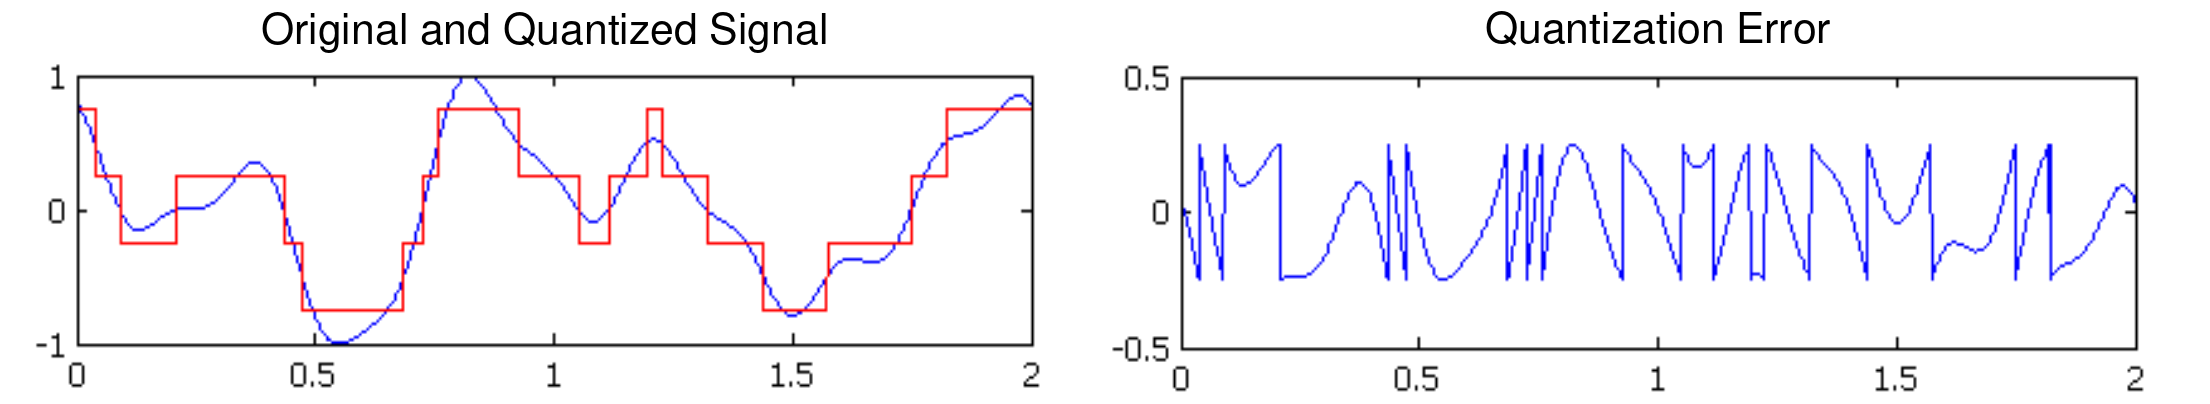
\includegraphics[width=\linewidth]{stanford_quantization_wide.png}
%   \end{minipage}%
%   \caption{Example of a quantized waveform.}
%   \label{fig:quantization}
% \end{figure}

\section{Experiment}
Lorem ipsum ...

\subsection{Tested Compressors}
.......

\section{Results \& Discussion}
Lorem ipsum ...


\section{Conclusions}

After completing the assignment, we drew a few conclusions regarding our 
solutions and ..................

Lorem ipsum ...

In terms of code organization and readability, we made sure our 
repository was as well structured as possible and our code properly commented
and documented.
The base folder contains a {\it README\/} file for basic instructions.
All code is in the {\it src\/} folder.

\newpage
\begin{thebibliography}{9}
  \bibliographystyle{Science}

  \bibitem{trab3}
    Armando J. Pinho,
    \textit{AIT: Lab Work no.3},
    University of Aveiro,
    2019/20.
  
\end{thebibliography}

\clearpage

\end{document}




















